\documentclass[spanish, 11pt]{article}

\usepackage[T1]{fontenc}
\usepackage[spanish]{babel}
\usepackage[letterpaper, margin=2.54cm]{geometry}
\usepackage{
    graphicx,
    amssymb, 
    amsmath,
    xltabular,
    booktabs,
    array,
    setspace,
    hyperref,
    fancyhdr
    }

\onehalfspacing
\decimalpoint
\setlength{\columnsep}{2cm}
\setlength{\parindent}{0cm}
\pagestyle{plain}
\hyphenpenalty=10000
\exhyphenpenalty=10000
\sloppy

\fancypagestyle{plain}{
    \fancyhead[L]{\textsc{Física General}}
    \fancyhead[R]{\textit{Estática}}
    \renewcommand{\headrulewidth}{0pt}
    \renewcommand{\footrulewidth}{0pt}
}

\title{\textbf{Cálculo de un vector resultante}}
\author{Rosendo Camal \\
    Universidad Aztlán \\
    \url{rosendocamal.edu@gmail.com}
    }
\date{13 de noviembre de 2026}

\begin{document}
\maketitle

\begin{table}[!htb]
    \centering
    \begin{tabular}{p{1cm}p{1.5cm}p{1cm}p{3.1cm}p{3.1cm}}
        \toprule
         & \textbf{Fuerza ($F$, N)} & \textbf{$\theta$ (Ángulo)} & \textbf{Componente $F_x = F \cos{\theta}$ (N)} & \textbf{Componente $F_y = \sin{\theta}$ (N)} \\
        \midrule
        $F_1$ & 50 N & 30° & 43.3 & 25 \\
        $F_2$ & 80 N & 120° & -40 & 69.28 \\
        $F_3$ & 40 N & 225° & -28.28 & -28.28 \\
        $F_4$ & 60 N & 315° & 42.43 & -42.43 \\
        \midrule
        \textbf{Total} & \multicolumn{2}{c}{\textbf{Suma de componentes ($\Sigma$)}} & 17.45 & 23.57 \\
        \bottomrule
    \end{tabular}
    \caption{Tabla de Componentes de Fuerza}
    \label{tab:componentes-fuerza}
\end{table}

El vector \textbf{resultante} es \(R = \bigl(\begin{smallmatrix}17.45 \\ 23.57\end{smallmatrix}\bigr)\).

\begin{figure}[!htb]
    \centering
    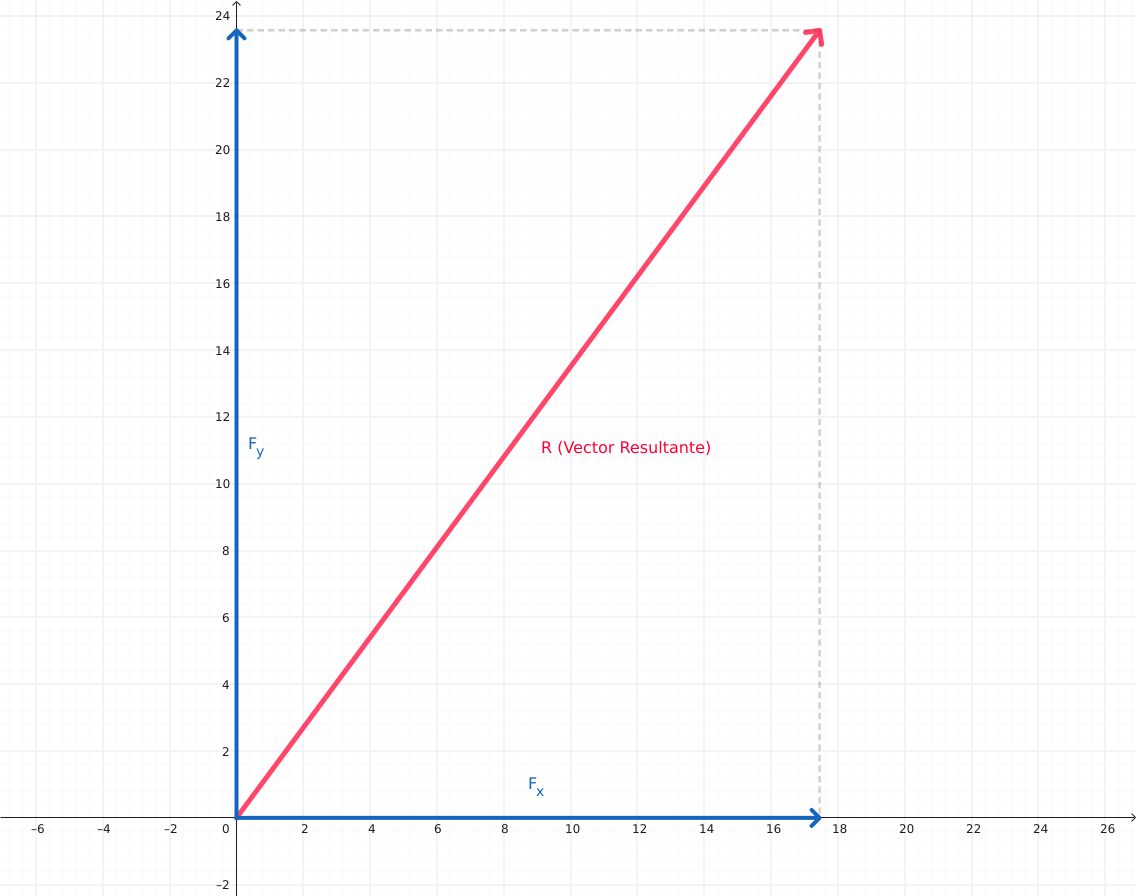
\includegraphics[scale=0.3]{geogebra-export.png}
    \caption{\textit{Diagrama Vectorial del Triángulo Final y Cálculo de Fuerza Resultante}}
\end{figure}


La \textbf{magnitud} de la resultante es \(R = \sqrt{(\Sigma F_x)^{2} + (\Sigma F_y)^{2}} = 29.33\).

La \textbf{dirección} de la resultante es \(\theta_R = \arctan\left(\frac{\Sigma F_y}{\Sigma F_x}\right) = 53.49^\circ\).


\end{document}